\section{Type system}

\begin{figure}[htbp]
    \centerline{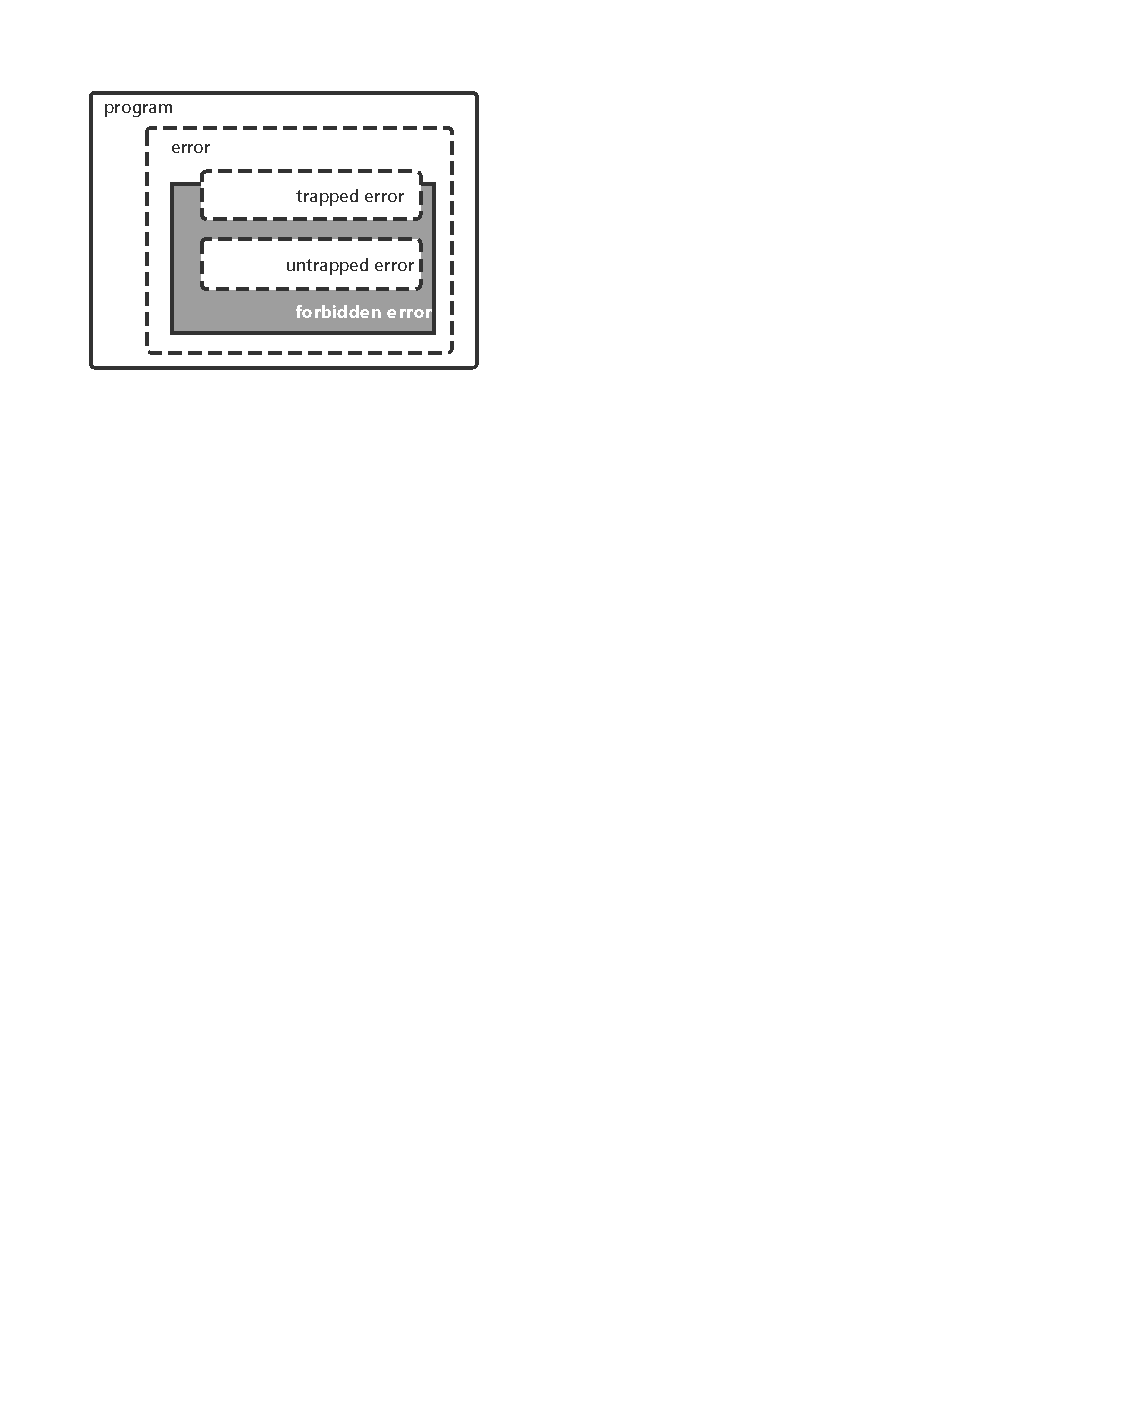
\includegraphics[scale=0.8]{figures/type-definition}}
    \caption{type-definition}
    \label{fig:type-definition}
\end{figure}


For definitional precision, the type system definition of L Cardelli is adopted here. This definition assumes that the fundamental purpose of the type system is to prevent errors that occur during the operation of a program, and therefore defines the type system by defining the concepts associated with errors. First defining what an error is to define good behavior. Then, according to the timing of behavior checking, it is divided into dynamic checking and static checking. On the basis of static checking, strong type checking and weak type checking are divided by whether forbidden error can be checked or not. As for the actual types in programming languages, they are divided into typed (static) languages and untyped (static) languages based on whether or not static types exist to limit the scope of runtime variables. Explicitly typed languages and implicitly typed languages are further divided according to whether the type of the variable is explicitly specified or not.

A very confusing issue is that the definition of the type system of programming languages varies from context to context. And there is a part of the population that discusses the types of programming languages without specifying the definition of the type system, which can easily lead to meaningless arguments about the type system in practice. A part of the population believes that JavaScript is a dynamic, weakly typed language, not an untyped language as judged here. This way of judging is also correct. In fact, the definition of this judgment criterion is based on values and variables, not on error checking as here. Another thing worth discussing is Python. type hints were introduced in Python in version 3.5. but in fact type hints do not actually error check Python, but are merely a type annotation to help provide better support for static analysis syntax parsers. The real time for error checking is still at runtime.


\begin{table*}[ht]
    \caption{type}
    \label{tab:type}
    \begin{center}
        \begin{tabular}{cccccc}
            \toprule
            Language & Typed/Untyped & Explicitly/Implicitly typed &
            Dynamically/Statically checked & Strongly/Weakly checked & Well behaved\\
            \midrule
            Python     & Typed   & Implicitly & Dynamically & Strongly & Yes \\
            Java       & Typed   & Explicitly & Statically  & Strongly & Yes \\
            C++        & Typed   & Explicitly & Statically  & Weakly   & No  \\
            JavaScript & Untyped & -          & Dynamically & -        & Yes \\
            Go         & Typed   & Explicitly & Statically  & Strongly & Yes \\
            Swift      & Typed   & Explicitly & Statically  & Strongly & Yes \\
            Dart       & Typed   & Explicitly & Statically  & Strongly & Yes \\
            Rust       & Typed   & Explicitly & Statically  & Strongly & Yes \\
            Kotlin     & Typed   & Explicitly & Statically  & Strongly & Yes \\
            \bottomrule
        \end{tabular}
    \end{center}
\end{table*}

The role of the type system for programming languages is obvious.

\begin{enumerate}
    \item Reduced expressiveness. Compared to untyped languages, the expressiveness of typed languages is somewhat reduced. But expressiveness can be improved by increasing the complexity of the type system, such as paradigms, union types, etc.
    \item Improved maintainability. Type signatures contain constraint information, and the function of a variable or function can be indirectly determined by the type signature.
    \item Improved reliability. First, the type system provides a means to check for errors. Second, the correctness of a program can be proved formally by the type system.
    \item Improved performance. First, untyped languages incur additional performance overhead at runtime for type checking and conversion. Second, typelessness is not conducive to compilation optimization. Some common JIT optimizations such as loop expansion are difficult to perform in untyped languages. Third, untyped memory memory allocation is more inefficient.
\end{enumerate}

